\section{问题四模型建立与求解}
\label{sec:question4}

\subsection{问题四分析}

问题四将固定分时电价改为未知交易电价，分别推广日前采购与滚动策略。五倍紧急补购使高价时的缺口损失更大，采购须共同考虑价格与净负荷的波动。

本问沿用储能约束与结算口径，以价格加权分位数解释联合建模，再用同日残差生成价荷场景。日前版保留母模型，滚动版沿用第\ref{sec:q3_candidate_screening}节的全时点筛选，实际账单按附件4已实现价格结算。

\subsection{问题四模型建立}

\begin{modelsummary}{问题四模型汇总}
\textbf{输入：}合法价荷预测、同日配对残差、当前SOC与有效合同。\par
\textbf{决策：}日前版求共同购电计划，滚动版在四个交易时点回放筛选采购候选。\par
\textbf{目标：}最小化配对情景下计划、调整、紧急费用与终端库存项的加权和。\par
\textbf{约束与输出：}沿用供需不等式、储能界与计划量结算规则，输出两版购电、充放电、紧急补购及按实际价格结算的账单。
\end{modelsummary}

\subsubsection{价格与需求相关时的采购分位数}

先考虑无储能单时段子问题。设未来净需求$X$与未来结算电价$P$可能相关，日前在已有信息下固定$q\ge0$；假设$P>0$几乎处处成立、$0<\mathbb E[P]<\infty$、$\mathbb E[PX_+]<\infty$，且富余购电无残值。期望费用为
\begin{equation}
 J_4(q)=\mathbb E[P]q+5\mathbb E[P(X-q)_+],\qquad q\ge0.
 \label{eq:mech_q4_cost}
\end{equation}
为保留$P$与缺口$(X-q)_+$的关联，定义
\begin{equation}
 \begin{cases}
 G(x)=\dfrac{\mathbb E[P\,\mathbf 1_{\{X\le x\}}]}{\mathbb E[P]},\\[6pt]
 G(x^-)=\dfrac{\mathbb E[P\,\mathbf 1_{\{X<x\}}]}{\mathbb E[P]}.
 \end{cases}
 \label{eq:mech_weighted_cdf}
\end{equation}
正价与有限期望保证$G$是合法分布函数。式\eqref{eq:mech_q4_cost}为凸函数，其次梯度为
\begin{equation}
 \partial J_4(q)=\mathbb E[P][5G(q^-)-4,\ 5G(q)-4].
 \label{eq:mech_q4_subgradient}
\end{equation}
内点最优条件为$G(q^-)\le0.8\le G(q)$，若最优点处连续，则
$\mathbb E[P\mathbf 1_{\{X\le q\}}]/\mathbb E[P]=0.8$。结合非负约束，可取
\begin{equation}
 q_4^\star=\max\{0,G^{-1}(0.8)\}.
 \label{eq:mech_weighted_quantile}
\end{equation}
对于离散场景$(x_s,p_s,\pi_s)$，只需把概率改写为
\begin{equation}
 \begin{cases}
 \widetilde\pi_s=\dfrac{\pi_sp_s}{\sum_j\pi_jp_j},\\[6pt]
 G(x)=\displaystyle\sum_{s:x_s\le x}\widetilde\pi_s.
 \end{cases}
 \label{eq:mech_scenario_reweight}
\end{equation}
无储能单时段的最优采购对应价格加权需求的80\%分位数。价荷独立时$G=F_X$，退化为普通分位数；高需求伴随高价时，其经济权重上升。完整调度进一步联合处理储能容量、效率、功率及跨时段能量价值。

\subsubsection{合法价格预测与同日价荷残差场景}

负荷与光伏沿用问题二、三的配置，价格预测器经一月验证后冻结：日前版采用最近四个同星期日价格均值，滚动版采用最近两个。日前负荷取最近两个同星期日均值、光伏取近三日均值；滚动版采用已发布光伏预报及负荷偏差反馈。

滚动版在$\tau>0$时按式\eqref{eq:q3_load_bias}、\eqref{eq:q3_load_update}修正价格：取此前12段实价相对零时预测的均值偏差，按六小时尺度衰减，限幅$\pm30\%$，预测下界为$10^{-6}$元/kWh。

对过去完整日$j<D$，分别求同发布时间的净负荷残差$\epsilon^n_{j,t}$和价格残差
\begin{equation}
 \epsilon^p_{j,t}=p_{j,t}-\widehat p^{(\tau)}_{j,t},\qquad t\ge\tau.
 \label{eq:q4_price_residual}
\end{equation}
两类残差按同一历史日配对，构成
\begin{equation}
 \begin{cases}
 n_{t,s}=\widehat n_t+\epsilon^n_{j_s,t},\\[2pt]
 p_{t,s}=\max\{0.01,\widehat p_t+\epsilon^p_{j_s,t}\}.
 \end{cases}
 \label{eq:joint_scenario}
\end{equation}
主案等权保留至多28日完整配对轨迹，同时保存连续误差与价荷联系。12场景对照先分别标准化净负荷与价格残差块，再按轨迹距离选择代表日。

场景价下界0.01元/kWh用于外层合成，实际结算仍保留原始最低价0.0076元/kWh。图\ref{fig:q4-correlation}描述2--12月48096段的Pearson相关：净负荷与价格的实际值相关系数为0.2620，按当时合法预测计算的残差相关系数为0.3468，显示配对场景所保留的样本联系。

\begin{figure}[htbp]\centering
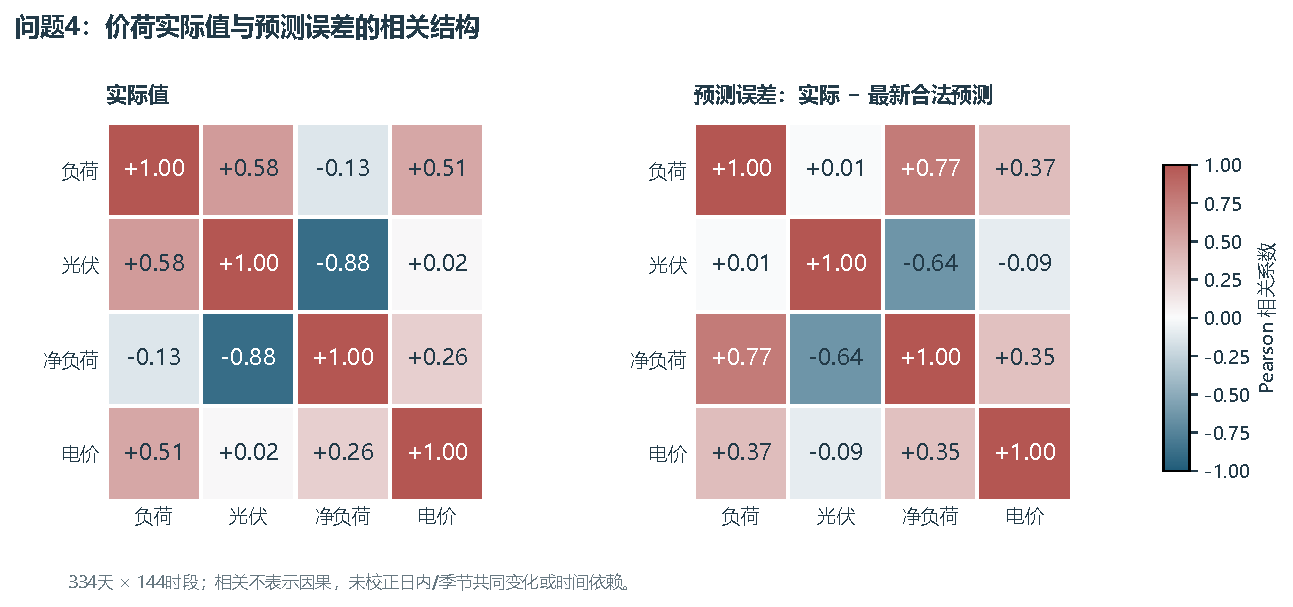
\includegraphics[width=0.91\linewidth]{figures/results/q4_correlation_heatmap.pdf}
\caption{滚动配置48096段的描述性Pearson相关矩阵：负荷、光伏、净负荷和电价。左为实际值，右为相对最近合法预测的误差，四次预报各覆盖36段；色标为$-1$至1。}
\label{fig:q4-correlation}
\end{figure}

\subsubsection{动态日前采购与动态滚动采购的共同优化结构}

在每个外层时点，记$\bar p_t=\sum_s\pi_sp_{t,s}$，共享参考储能仍为$c_t,d_t,e_{t+1}$，紧急补购为$h_{t,s}$。动态日前案在零时求解
\begin{equation}
 \min\left\{\sum_{t=0}^{143}\bar p_tg_t+
  \sum_s\pi_s\sum_{t=0}^{143}5p_{t,s}h_{t,s}
  +\beta_T|e_{144}-6000|\right\},
 \label{eq:q4_day_ahead_objective}
\end{equation}
满足式\eqref{eq:scenario_balance}及储能约束，初态承接当日实际库存。常规采购按场景均价评价，紧急费用逐场景乘对应价格。

滚动母模型零时采用式\eqref{eq:q4_day_ahead_objective}，6、12、18时采用式\eqref{eq:q3_revision_objective}--\eqref{eq:q3_revision_contract}的联合场景价格版本。最终方案在四个时点将该LP与点预测、三个余量及日内当前合同候选统一筛选。回放保持同日价格--净负荷配对，紧急费为$5p_{t,s}h_{t,s}^{(k)}$，计划费与调整费也按对应情景价格计算；所有候选共用加权价格序列的中位数作为终端系数。

实际费用按式\eqref{eq:settlement}及附件4已实现价格结算。日前版$a_t=g_t$，滚动版按合法时点修订，原计划均按计划量全额付费。两版按实际供需执行储能并连续传递SOC，回放方法沿用问题三。

主案预设$\lambda=0$、$\rho_t=0$。母模型的内层LP对照使用当期实价与后续合法预测，固定合同和跨日临时变量的定义沿用问题三。

\subsection{问题四求解}

\subsubsection{最终配置与实际求解步骤}

未筛选母模型的一月验证中，日前规则费用1042234.20元，LP为1052652.76元；滚动规则为1043044.13元，剩余日LP为1057597.78元，LP加跨日为1047012.91元（表\ref{tab:v2_controller_validation}），两版据此冻结规则执行器。表\ref{tab:outer_timing_ablation}的筛选比较确定滚动版采用全时点配置；日前版启用筛选增费0.428\%，保留母模型。

求解依次完成配对场景构造、采购决策、实际供需下的储能执行与分项结算。日前和滚动版的2月初始SOC分别为9251.54、9030.40 kWh，均承接各自固定的一月运行前缀。

\subsubsection{全年费用与紧急补购权衡}

动态日前案334天计划费用14280142.03元、紧急费用513982.26元，总费用14794124.29元，紧急量80544.00 kWh，涉及106天、596个十分钟时段。最终动态滚动案计划费用14265228.71元、调整费用283142.26元、紧急费用121866.90元，总费用14670237.87元，紧急量21293.41 kWh，涉及116天、418个十分钟时段。两案总费用相差123886.42元，即滚动案低0.8374\%，紧急量低73.56\%。

图\ref{fig:q4-cost-waterfall}按未舍入账单分解两版费用差：滚动版计划费减少14913.32元、紧急费减少392115.36元，新增调整费283142.26元。

\begin{figure}[htbp]\centering
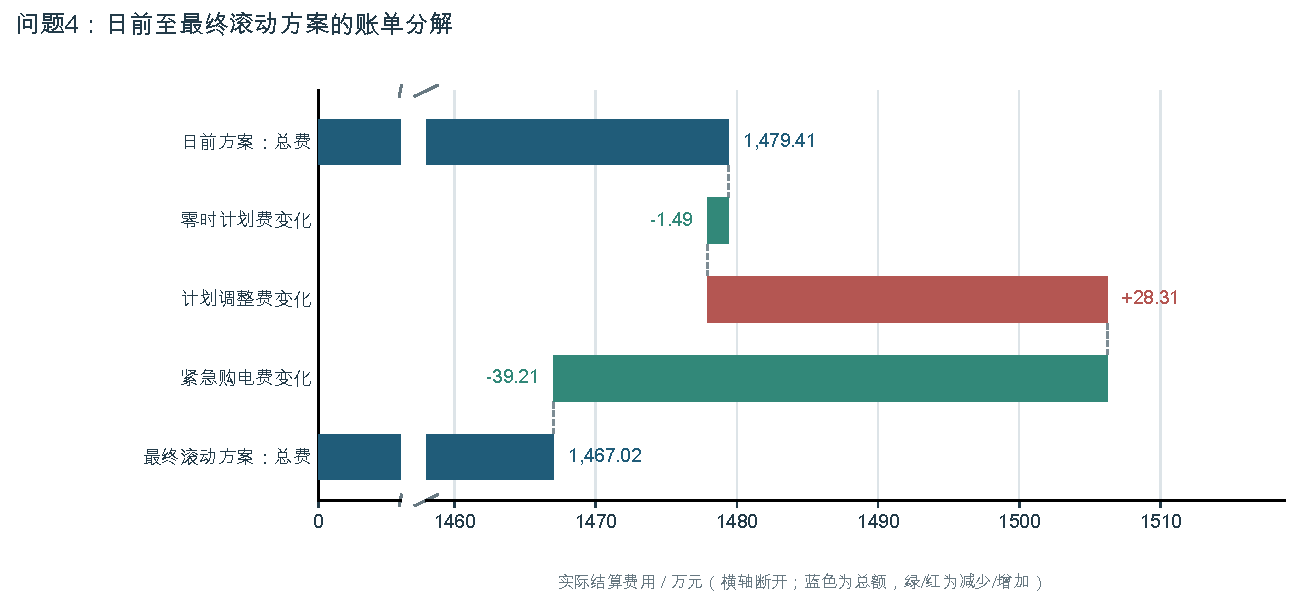
\includegraphics[width=0.95\linewidth]{figures/results/q4_cost_waterfall.pdf}
\caption{日前母模型到全时点筛选滚动版的整体账单差（万元）。起止条从零累计至334天总费，中间条为计划、调整与紧急费变化，断轴放大差异。}
\label{fig:q4-cost-waterfall}
\end{figure}

滚动版与日前版的实际日费用CVaR95分别为77575.87元、83044.31元，最高日费用分别为81797.18元、108080.37元，期末库存分别为6274.99、6269.86 kWh。CVaR以334个实际日账单计算，描述尾部费用。

以未筛选滚动母模型14769232.53元为同条件基线，全时点筛选节省98994.66元，紧急量增加9342.73 kWh，日费用CVaR95由77420.84升至77575.87元（表\ref{tab:outer_timing_ablation}、\ref{tab:outer_screening_tradeoff}），体现总费用与补购需求、尾部费用的权衡。

\subsubsection{指定日期采购、储能与紧急购电结果}

以下给出两版最终配置在四个指定日的六个时段采购量、全天常规量、四小时储能汇总及紧急区间。电量以kWh计，实际费用含紧急补购，计划费与调整费另行分解。表格与工作簿均按统一物理索引读取最终执行数组，保留原模板显示标签。

\begin{table}[!htbp]\centering\small
\caption{问题四日前版指定日期购电结果（电量：kWh）}
\label{tab:q4_2-purchase}
\setlength{\tabcolsep}{4pt}
\begin{tabularx}{\linewidth}{lRRRR}\toprule
物理时段 & 03-20 & 06-21 & 09-23 & 12-21\\\midrule
10:00--10:10 & 0.00 & 0.00 & 0.00 & 0.00\\
12:00--12:10 & 564.20 & 0.00 & 497.24 & 970.92\\
14:00--14:10 & 0.00 & 0.00 & 0.00 & 0.00\\
16:00--16:10 & 490.32 & 296.43 & 537.29 & 851.12\\
18:00--18:10 & 0.00 & 510.07 & 0.00 & 744.23\\
20:00--20:10 & 743.27 & 0.00 & 0.00 & 0.00\\
\midrule
全天常规量 & 67869.67 & 40675.72 & 69762.68 & 100945.95\\
全天实际费用/元 & 42207.16 & 21012.94 & 48309.88 & 77020.40\\
\bottomrule\end{tabularx}
\par\smallskip\parbox{\linewidth}{\footnotesize 日期均为2025年；购电量为零时计划量，紧急量单列。实际费用包含计划、调整及紧急三项账单。}
\end{table}

\begin{table}[!htbp]\centering\fontsize{10}{12}\selectfont
\caption{问题四日前版指定日期储能结果（kWh）}
\label{tab:q4_2-battery}
\setlength{\tabcolsep}{4pt}
\begin{tabularx}{\linewidth}{lRRRR}\toprule
物理时段 & 03-20 & 06-21 & 09-23 & 12-21\\\midrule
00:00--04:00 & 3824.42 / 134.84 & 963.51 / 3780.66 & 5330.27 / 22.20 & 4499.29 / 40.16\\
04:00--08:00 & 1669.83 / 5857.47 & 1400.69 / 1719.95 & 206.94 / 5820.07 & 0.00 / 741.76\\
08:00--12:00 & 6146.04 / 2777.38 & 6932.04 / 0.00 & 5946.19 / 1896.62 & 5940.70 / 6486.91\\
12:00--16:00 & 3907.13 / 420.71 & 0.00 / 0.00 & 3587.87 / 530.87 & 5724.46 / 2220.11\\
16:00--20:00 & 174.78 / 6369.00 & 0.00 / 4853.45 & 163.52 / 6562.31 & 0.00 / 5500.96\\
20:00--24:00 & 5798.62 / 2212.03 & 7501.98 / 3091.92 & 5525.15 / 1842.66 & 5818.48 / 2842.53\\
\midrule
期初 / 期末库存 & 6834.43 / 6457.15 & 8545.17 / 8723.59 & 6002.76 / 6159.23 & 6795.26 / 6766.10\\
\bottomrule\end{tabularx}
\par\smallskip\parbox{\linewidth}{\footnotesize 六个时段行按“充电量 / 放电量”列示；末行为当日0时 / 24时库存。}
\end{table}

\begin{table}[!htbp]\centering\small
\caption{问题四日前版指定日期紧急购电}
\label{tab:q4_2-emergency}
\setlength{\tabcolsep}{4pt}
\begin{tabularx}{\linewidth}{lLR}\toprule
日期 & 物理区间 & 紧急电量/kWh\\\midrule
03-20 & 无 & 0.00\\
06-21 & 无 & 0.00\\
09-23 & 18:20--18:40 & 3.91\\
 & 20:30--20:40 & 357.19\\
 & 20:50--21:10 & 90.05\\
 & 21:20--21:50 & 34.20\\
12-21 & 无 & 0.00\\
\midrule
四日合计 &  & 485.35\\
\bottomrule\end{tabularx}
\par\smallskip\parbox{\linewidth}{\footnotesize 各日合计依次为0.00、0.00、485.35、0.00 kWh。}
\end{table}

\begin{table}[htbp]\centering\small
\caption{问题4-2指定日期计划、调整与费用分解}
\begin{tabularx}{\linewidth}{lRRRRR}\toprule
日期 & 计划量/kWh & 生效量/kWh & 计划费/元 & 调整费/元 & 紧急费/元\\\midrule
2025-03-20 & 67869.67 & 67869.67 & 42207.16 & 0.00 & 0.00\\
2025-06-21 & 40675.72 & 40675.72 & 21012.94 & 0.00 & 0.00\\
2025-09-23 & 69762.68 & 69762.68 & 45194.04 & 0.00 & 3115.84\\
2025-12-21 & 100945.95 & 100945.95 & 77020.40 & 0.00 & 0.00\\
\bottomrule\end{tabularx}\end{table}
\FloatBarrier
\begin{table}[!htbp]\centering\small
\caption{问题四滚动版指定日期购电结果（电量：kWh）}
\label{tab:q4_3-purchase}
\setlength{\tabcolsep}{4pt}
\begin{tabularx}{\linewidth}{lRRRR}\toprule
物理时段 & 03-20 & 06-21 & 09-23 & 12-21\\\midrule
10:00--10:10 & 0.00 & 0.00 & 22.75 & 0.00\\
12:00--12:10 & 624.29 & 0.00 & 461.07 & 1054.19\\
14:00--14:10 & 0.00 & 0.00 & 54.35 & 0.00\\
16:00--16:10 & 671.04 & 260.52 & 611.01 & 877.48\\
18:00--18:10 & 704.20 & 495.32 & 0.00 & 744.23\\
20:00--20:10 & 743.27 & 0.00 & 822.11 & 0.00\\
\midrule
全天常规量 & 71574.04 & 37518.90 & 73431.36 & 101918.89\\
全天实际费用/元 & 45107.31 & 19308.93 & 47890.72 & 77624.69\\
\bottomrule\end{tabularx}
\par\smallskip\parbox{\linewidth}{\footnotesize 日期均为2025年；购电量为最终生效常规量，紧急量单列。实际费用包含计划、调整及紧急三项账单。}
\end{table}

\begin{table}[!htbp]\centering\fontsize{10}{12}\selectfont
\caption{问题四滚动版指定日期储能结果（kWh）}
\label{tab:q4_3-battery}
\setlength{\tabcolsep}{4pt}
\begin{tabularx}{\linewidth}{lRRRR}\toprule
物理时段 & 03-20 & 06-21 & 09-23 & 12-21\\\midrule
00:00--04:00 & 4119.21 / 134.84 & 675.55 / 4135.87 & 5172.38 / 22.20 & 4436.14 / 40.16\\
04:00--08:00 & 825.23 / 5868.37 & 1424.39 / 1719.95 & 177.31 / 5680.26 & 735.70 / 1384.74\\
08:00--12:00 & 5765.88 / 2777.38 & 8481.89 / 0.00 & 6536.73 / 1893.23 & 6412.06 / 6391.52\\
12:00--16:00 & 5187.95 / 254.72 & 0.00 / 0.00 & 3099.44 / 353.23 & 5218.63 / 2240.52\\
16:00--20:00 & 28.20 / 6553.40 & 0.00 / 5210.22 & 96.08 / 6443.21 & 0.00 / 5490.42\\
20:00--24:00 & 5792.33 / 1970.23 & 6461.65 / 2485.90 & 5603.57 / 2259.51 & 5769.36 / 2842.53\\
\midrule
期初 / 期末库存 & 6530.78 / 6567.77 & 7782.84 / 8064.24 & 6144.86 / 6260.00 & 6852.09 / 6733.60\\
\bottomrule\end{tabularx}
\par\smallskip\parbox{\linewidth}{\footnotesize 六个时段行按“充电量 / 放电量”列示；末行为当日0时 / 24时库存。}
\end{table}

\begin{table}[!htbp]\centering\small
\caption{问题四滚动版指定日期紧急购电}
\label{tab:q4_3-emergency}
\setlength{\tabcolsep}{4pt}
\begin{tabularx}{\linewidth}{lLR}\toprule
日期 & 物理区间 & 紧急电量/kWh\\\midrule
03-20 & 无 & 0.00\\
06-21 & 无 & 0.00\\
09-23 & 18:30--18:40 & 2.38\\
 & 20:10--20:20 & 10.23\\
12-21 & 无 & 0.00\\
\midrule
四日合计 &  & 12.61\\
\bottomrule\end{tabularx}
\par\smallskip\parbox{\linewidth}{\footnotesize 各日合计依次为0.00、0.00、12.61、0.00 kWh。}
\end{table}

\begin{table}[htbp]\centering\small
\caption{问题4-3指定日期计划、调整与费用分解}
\begin{tabularx}{\linewidth}{lRRRRR}\toprule
日期 & 计划量/kWh & 生效量/kWh & 计划费/元 & 调整费/元 & 紧急费/元\\\midrule
2025-03-20 & 71574.04 & 71574.04 & 45107.31 & 0.00 & 0.00\\
2025-06-21 & 37505.63 & 37518.90 & 19288.01 & 20.91 & 0.00\\
2025-09-23 & 73403.01 & 73431.36 & 47750.49 & 57.78 & 82.45\\
2025-12-21 & 101918.89 & 101918.89 & 77624.69 & 0.00 & 0.00\\
\bottomrule\end{tabularx}\end{table}
\FloatBarrier

\subsubsection{跨月份表现}

图\ref{fig:v2-monthly}汇总四组最终配置的月度费用与紧急量：日前两组保留母模型，滚动两组采用全时点筛选。月度波动反映季节负荷、光伏、价格和历史误差的共同变化。

\begin{figure}[H]\centering
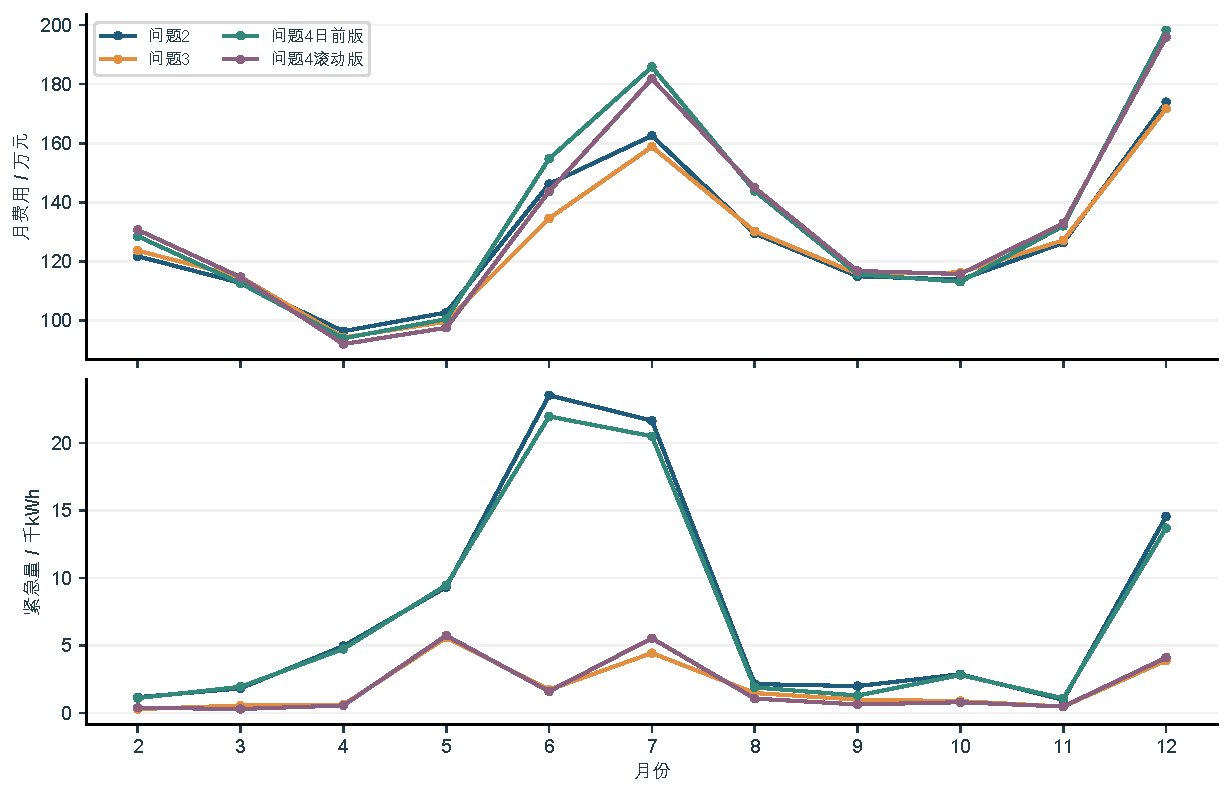
\includegraphics[width=0.95\linewidth]{figures/results/v2_monthly.pdf}
\caption{四组最终配置的月度实际费用与紧急量，按逐日账单和执行电量求和。日前两组采用母模型，滚动两组采用全时点筛选。}
\label{fig:v2-monthly}
\end{figure}

联合场景使采购反映缺口与价格的共同风险，储能和滚动修订处理跨时段与信息更新。全时点候选筛选取得本次四种启用配置中的最低总费用。
\FloatBarrier
